\subsection{Tunnels and caverns}
The detector topology for a wide-band gravitational wave observatory must adopt a xylophone detection scheme containing six interferometers housed in triangular configuration. Fig. \ref{Landscape} shows a scaled impression of the underground observatory. Each xylophone detector will be centered around one of the corner stations and is composed of a high and low frequency interferometer pair. The first step in a phased approach towards realisation of Einstein Telescope is the construction of the full underground infrastructure including a single xylophone detector. 

Presently, it is not clear whether the observatory will have horizontal or vertical access. When considering sites, the manner in which access to the underground facilities is allowed, requires careful consideration. In traditional mining, access to the underground is via a decline (ramp) or inclined vertical shaft, or adit. Shafts are considered as vertical excavations while adits are horizontal excavations into the side of a hill or mountain. 

An important consideration is that the realization of direct vertical access shafts to depths exceeding 200\,m (which may be desirable for Einstein Telescope) carries with it construction methods that are significantly more complex than those needed for a more shallow infrastructure. All of these considerations tie in closely to the local geography and geology of a chosen site.
\begin{figure}[htbp!]
	\centering
		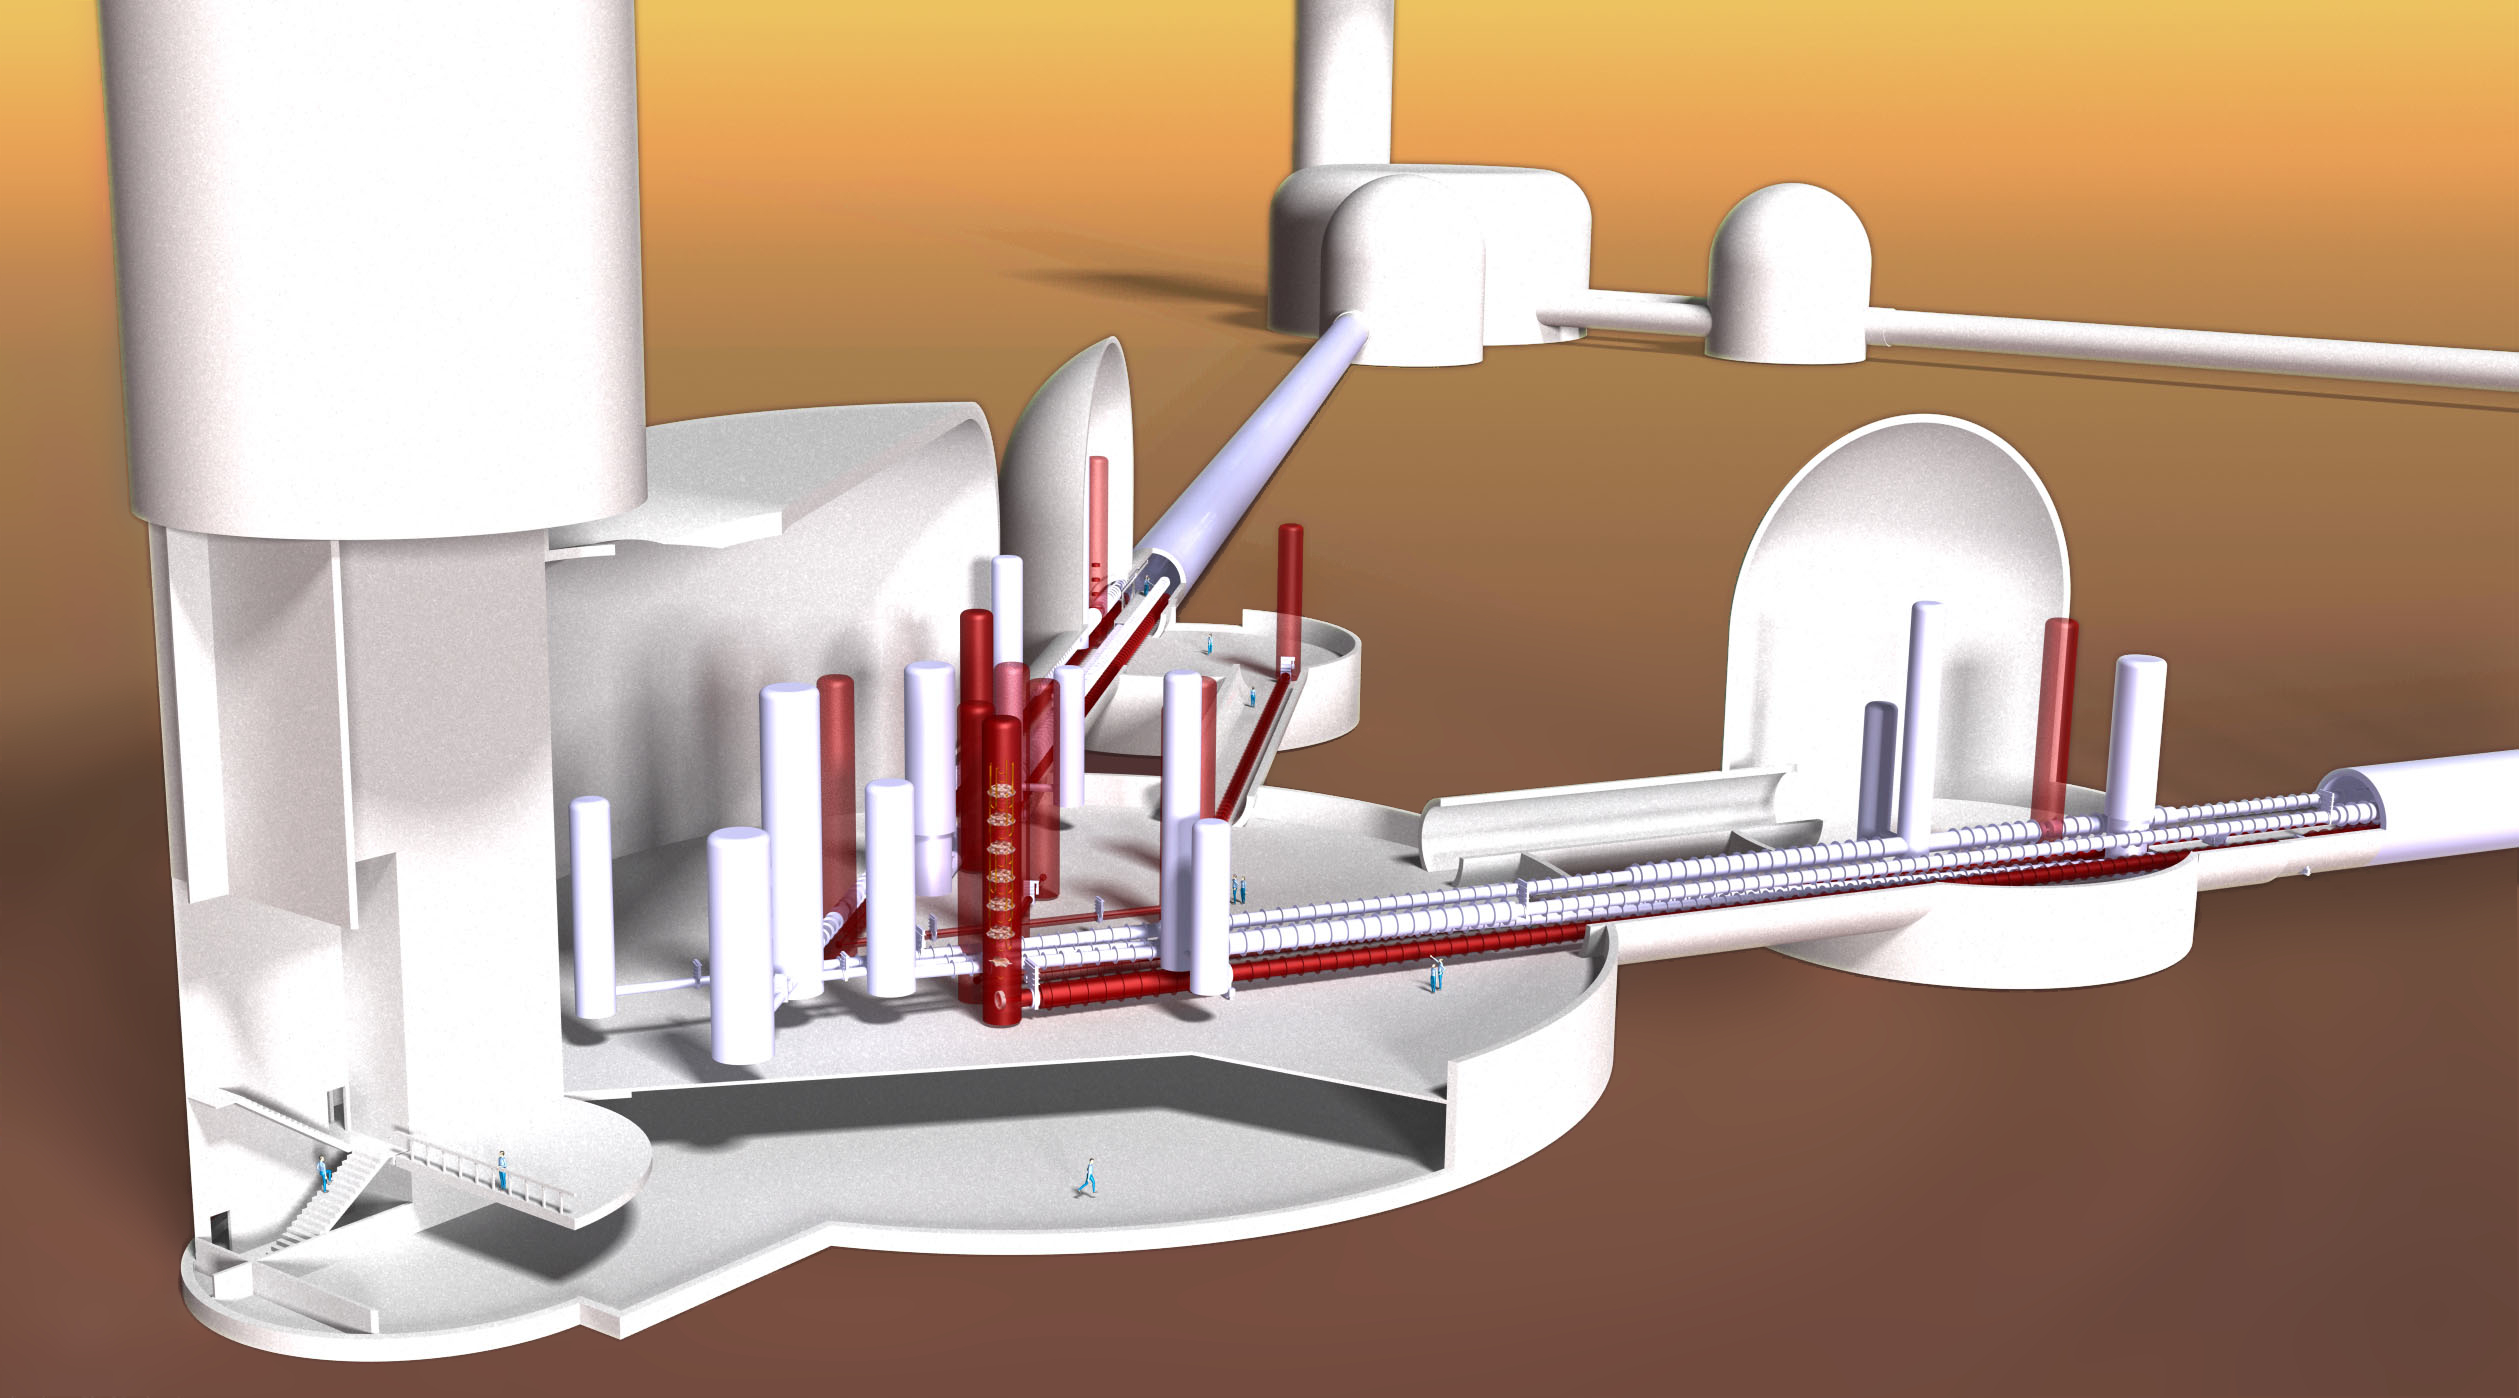
\includegraphics[width=17cm]{SiteInfra/TunnelsCaverns/TunnelsCavernsFigures/ShaftAccess.jpg}
		\caption{Impression of a corner station. Each station features a large cavern that can be accessed through a 20 m diameter vertical shaft. Two satellite caverns connect via twin tunnels to a main cavern and house input test masses and cryogenic infrastructure.}
	\label{shaftaccess}
\end{figure}

Figure \ref{shaftaccess} shows an impression of the observatory in case vertical access shafts are employed. Each corner station is built around a 20 m diameter vertical shaft. If tunnel excavation is accomplished by tunnel boring machines, then these will be lowered through these shafts at the start of construction. After tunnel construction, the shafts will be equipped with concrete elevator modules, staircases and will carry all services (power, water, compressed air, ventilation ducts, $etc.$). Additional shafts with a 10 m diameter are foreseen at the centre of the arms (not shown). The top of the shafts will be integrated in large surface buildings. There the equipment of the various interferometers, such as the vacuum system, will be prepared. Subsequently, the modules will be lowered through the shafts into the caverns by using hoisting devices.

{\it Each of the corner stations has a main cylindrical cavern with a 65\,m diameter (TBC)}. These caverns house the laser injection systems and many of the interferometer seismic isolation systems that suspend the optical components. Each cavern contains two levels. The top level has a height of 30\,m, required for housing the main suspension systems and their vacuum envelopes. The basement level contains 3.5\,m high passageways that lead to small cleanroom areas below the suspension systems, providing underneath access to the suspended optical components. The vacuum pipes for the low frequency and high frequency interferometer are situated on top of each other. In this way, the interferometer beams propagate horizontally and are housed in separate vacuum pipes. For cryogenic design purposes, the vacuum system of the cryogenic interferometer is situated on top of the high frequency system.

Each of the corner stations contains detector components from all three xylophone detectors. The main optical components of the interferometers need to be suspended requiring a total of 17 suspension towers in each main cavern. Four of these towers are part of the cryogenic suspension system for the end test masses. Finally, the main caverns are occupied by two cryolinks each, that protect the cryogenic end test masses from thermal radiation. 

An impression of a main- and a single satellite cavern, connected by a tunnel system is shown in Fig. \ref{infra}. It can be seen that the main cavern is connected to four tunnels. Two of these tunnels accommodate up to six vacuum beam pipes. A third tunnel holds a single vacuum pipe while the fourth tunnel is empty. This parallel tunnel system will be used to allow transportation of equipment between main caverns and auxiliary caverns, while providing parallel escape routes for emergency purposes.
\begin{figure}[h!]
    \centering
    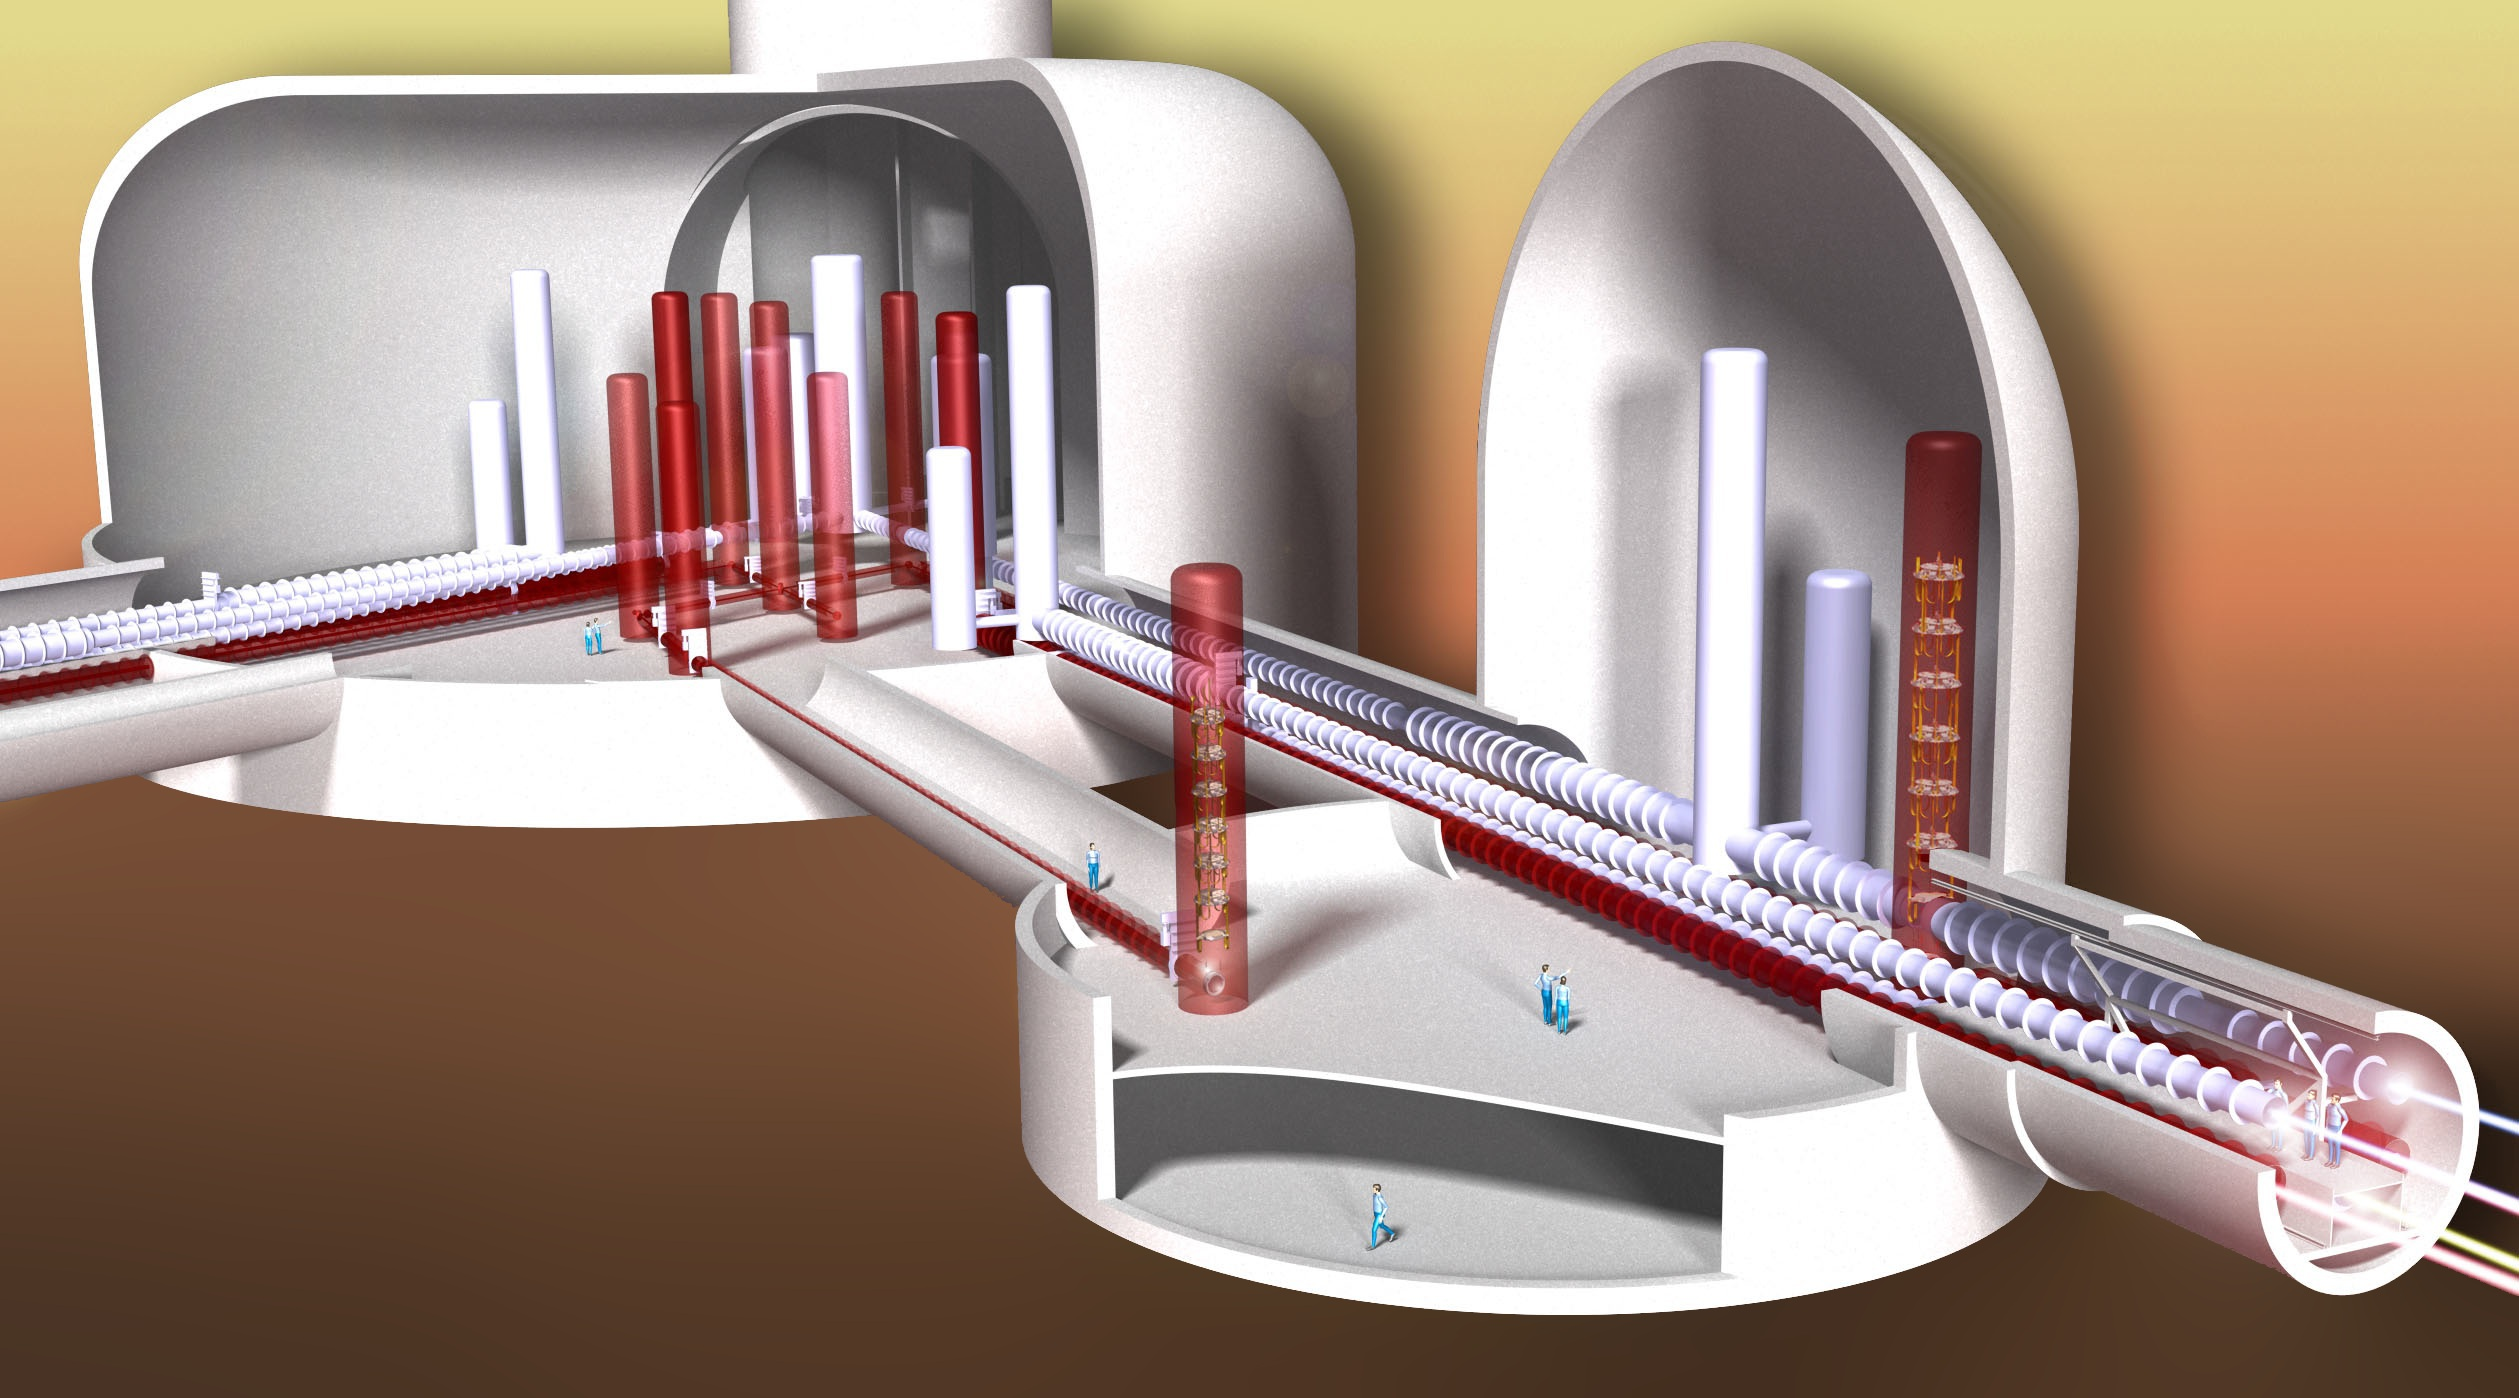
\includegraphics[width=17cm]{SiteInfra/TunnelsCaverns/TunnelsCavernsFigures/ArtisticView1.jpg}
    \caption{Impression of a corner station of Einstein Telescope. Satellite caverns are connected via double tunnels to the main caverns.  Filter cavities for the high frequency interferometer are placed in one of these tunnels. The satellite caverns house the input test masses and the cryogenics infrastructure.}
    \label{fig:infra}
\end{figure}
As with the main caverns, the satellite caverns contain two levels with 3.5\,m high passageways underneath the 30\,m high top level. These caverns are designed with a cylindrical in shape with an inner diameter of 30\,m. Although the inner diameter of the cavern could be optimised, the designed cavern provides flexibility and space for possible future infrastructure. In its final configuration, six beam pipes pass through this each of these caverns. The caverns are occupied by the input test masses of both the low frequency and high frequency interferometers. The low frequency input test masses are cryogenic payloads and are protected from thermal radiation by cryolinks. The satellite caverns are equipped with the necessary cryogenic infrastructure. 

The corner stations are connected by approximately 10 km long tunnels between the satellite caverns. {\it These tunnels have an inner diameter of 5.5\,m over most of their length (TBC)}. The main caverns and the auxilliary caverns are connected by parallel tunnels with a length of 300\,m. Consequently, in its final form the observatory will host more than 31 km of total tunnel length. The main interferometer arm tunnels accommodate six vacuum beam pipes: two for the high- and two for the low frequency interferometers, and two for filter cavities. In addition, the tunnel houses the services for electricity, water, compressed air, cryogenics, safety systems and air conditioning. 

During the construction of ET, the tunnel will be equipped with a monorail to transport sections of vacuum beam pipes to the welding and installation area. Later, this system is to be converted to a personnel transport system. For safety reasons the tunnel is divided into 500 m sections that are equipped with fire retarding doors, and safety shelters. The tunnel is equipped with an elaborate safety system that allows control of the airflow in order to direct the smoke in case of a fire.

Laser interferometers for gravitational wave detection require ultra-high vacuum systems for housing the optical systems. In order not to be limited by noise due to vacuum fluctuations, requires a base pressure below $10^{-10}$ mbar. Furthermore, the system must be extremely clean from organic molecules. Einstein Telescope will feature the world's largest ultra high vacuum system and in order to minimise costs, the beam pipes will be fabricated from stainless steel by continuous spiral welding. For this purpose, a dedicated clean factory will be installed on site.

Cryogenic infrastructure is needed for the operation of the various interferometers. Large cryo-traps are foreseen and will be cooled by liquid nitrogen in case of the high frequency interferometers. The cryo-plants required for the low frequency interferometer will provide refrigeration power allowing to bring the mirror temperatures to 4 K\footnote{Although the system allows cooling to 4 K, the system operates at 10 K.}. This can be accomplished by either a battery of cryo-coolers or by using liquid helium cryostats.

Safety and health will have the highest priority during every stage of the planning, design, construction, and operation of the observatory. Particular attention has to be paid to key areas such as underground communication, ventilation, access, emergency egress and refuge design. During the construction of the subterranean infrastructure, the safety of both engineering and scientific personnel has to be ensured. 

